% arara: pdflatex
% !arara: biber
% !arara: pdflatex
% How to run: 
% 1) pdflatex "filename".tex
% 2) biber "filename"
% 3) pdflatex "filename".tex
% 4) pdflatex "filename".tex


\documentclass[x11names]{article}
\usepackage{verbatim}
\usepackage{listings}
\usepackage{graphicx}
\usepackage{a4wide}
\usepackage{color}
\usepackage{amsmath}
\usepackage{amssymb}
\usepackage[dvips]{epsfig}
\usepackage[T1]{fontenc}
% \usepackage{cite} % [2,3,4] --> [2--4]
\usepackage{shadow}
\usepackage{hyperref}
\usepackage{physics}
\usepackage{url}
\usepackage{tikz}
\usepackage{subcaption}
\usepackage[utf8]{inputenc}
\usepackage{booktabs} % Allows the use of \toprule, \midrule and \bottomrule in tables
\usepackage[font={small,it}]{caption}
\usepackage[margin=0.7in]{geometry} %Sets the margins in the document
\usepackage{siunitx}    %Allows use of SI units macros

%Defines calculator way to write powers of ten
\sisetup{output-exponent-marker=\textsc{e}}


% Change numbering and some commands
\renewcommand\thesection{Exercise \Roman{section}}
\renewcommand\thesubsection{\Roman{section}.\alph{subsection}}

%% references
\usepackage[style=authoryear,
            bibstyle=authoryear,
            backend=biber,
            % refsection=chapter,
            maxbibnames=99,
            maxnames=2,
            firstinits=true,
            uniquename=init,
            natbib=true,
            dashed=false]{biblatex}

\addbibresource{bibliography.bib}
% \addbibresource{top.bib}

% \bibliography{bibliography}
% \bibliography{top}


\usepackage[capitalize]{cleveref}

\setcounter{tocdepth}{2}

\lstset{language=c++}
\lstset{alsolanguage=[90]Fortran}
\lstset{basicstyle=\small}
\lstset{backgroundcolor=\color{white}}
\lstset{frame=single}
\lstset{stringstyle=\ttfamily}
\lstset{keywordstyle=\color{red}\bfseries}
\lstset{commentstyle=\itshape\color{blue}}
\lstset{showspaces=false}
\lstset{showstringspaces=false}
\lstset{showtabs=false}
\lstset{breaklines}


\definecolor{keywords}{RGB}{255,0,90}
      \definecolor{comments}{RGB}{0,0,113}
      \definecolor{red}{RGB}{160,0,0}
      \definecolor{green}{RGB}{0,150,0}
       
      \lstset{language=Python, 
              basicstyle=\ttfamily\small, 
              keywordstyle=\color{keywords},
              commentstyle=\color{comments},
              stringstyle=\color{red},
              showstringspaces=false,
              identifierstyle=\color{green}
              }



\title{ Exercise 5 \\ Sommerjobb Numeriske Plasmaoppgaver }
\author{Gullik Vetvik Killie
		}


%%%%%%%%%%%%%%%%%%%%%%%%%%%%%%%%%%%%%%%%%%%%%%%%%%%%%%%%%%%%%%%%%%%%%%%%%%%%%%%%%%%%
% Actual text starts here
%%%%%%%%%%%%%%%%%%%%%%%%%%%%%%%%%%%%%%%%%%%%%%%%%%%%%%%%%%%%%%%%%%%%%%%%%%%%%%%%%%%%
\begin{document}


\maketitle

\section{Exercise}

\subsection{Theory}
  In this exercise we will examine the distribution of the electrostatic potential in the higher latitudes.

  In the high latitudes the plasma E\(\times\)B drifts in the ionosphere, assuming equilibrium in the atmosphere there is no accumulation of charges and \(\nabla\cdot\vb{E} = 0\). Then the electric field, caused by the plasma, can be represented as the gradient of an electrostatic potential \(\va{E} = - \nabla\Phi\). The electrostatic potential has a dependency on a scaled colatitude \(\theta\) and the longitude \(\phi\), but no dependence on the radial component and is best represented in terms of the associated Legendre polynomials \(P^m_\ell\).

  \begin{align}
    \Phi(\phi ,\theta) &= \sum^N_{\ell = 0}\sum^\ell_{m= 0} \left[ A_{\ell m}\cos(m \phi) + B_{\ell m}\sin(m \phi) \right] P^m_\ell(\cos(\theta))   \label{eq:phi_sum}
  \end{align}

  Where \(\ell\) and \(m\) is the degree and order respectively, while \(A_{\ell m}\) and \(B_{\ell m}\) are the spherical harmonic expansion coefficients. The the arguments of the Legendre polynomials \(\cos(\theta)\) is calculated as

  \begin{align}
    \cos(\theta) &= 2\frac{\lambda - 75^\circ}{30^\circ}, \text{  where the latitude }  \lambda \in [ 60^\circ, 90^\circ )
  \end{align}

  The harmonic coefficients can be found \href{http://folk.uio.no/lbnc/fys3610/heppner_coeffs.txt}{here}, courtesy of Lasse Clausen.


  \subsection{Computer program}
      A computer program that calculates the electrostatic potential is shown in \cref{sec:code} and returns a grid with it's values, on latitude and longitude coordinates. A pseudo-script explaining the workings of the program follows.

      \begin{enumerate}
        \item Prepare needed variables and arrays
        \item Read in the spherical harmonic expansion coefficients
        \item Fill \(A[l,m]\) and \(B[l,m]\)
          \begin{enumerate}
            \item For-loop over \(l\) and \(m\)
            \begin{itemize}
              \item Cycle trough the coefficients
              \item If the coefficients \(l\), \(m\) values is equal to both \(l\) and \(m\) place it in \(A[l,m]\) or \(B[l,m]\)
            \end{itemize}
          \end{enumerate}
        \item Then we calculate the arguments to the Legendre polynomials, \(\cos(\theta) = 2\frac{\lambda - 75^\circ}{30^\circ}\) and fills the legendre array with them.
              The first index of the legendre polynomial corresponds to which latitude we are at, and has a \(2D\) array connected to it since we need different values each \(l\) and \(m\)
        \item Then we fill the legendre \(3D\) array with entries using a scipy function lpmv( l, m, argument )
          \begin{itemize}
            \item Cycle through the latitudes, storing the argument
            \begin{itemize}
              \item Cycle through \(m\) and \(l\)
                \begin{itemize}
                  \item Calculate the entry using the function lpmv(l,m,argument) and store it in the legendre array at position \([ latitude_index, l, m ]\)
                \end{itemize}
            \end{itemize}
          \end{itemize}
        \item Set up a function \(\Phi( \phi, \text{Latitude Index}, text{Legendre Array} )\) which calculates the sum in \cref{eq:phi_sum}
        \item Then we cycle through the latitude and longitude grid and call the \(\Phi\) function to calculate the electrostatic potentials value at each entry
      \end{enumerate}


\subsection{Results}
  
  \cref{fig:potential} shows the electrostatic potential in the northen hemisphere. The magntitude of the potential varies between \(-24 \si{kV}\) and \(32 \si{kV}\). There is two poles vivisble on the potential representing the minimum and the maximum of the potential field.
  \begin{figure}
    \centering
    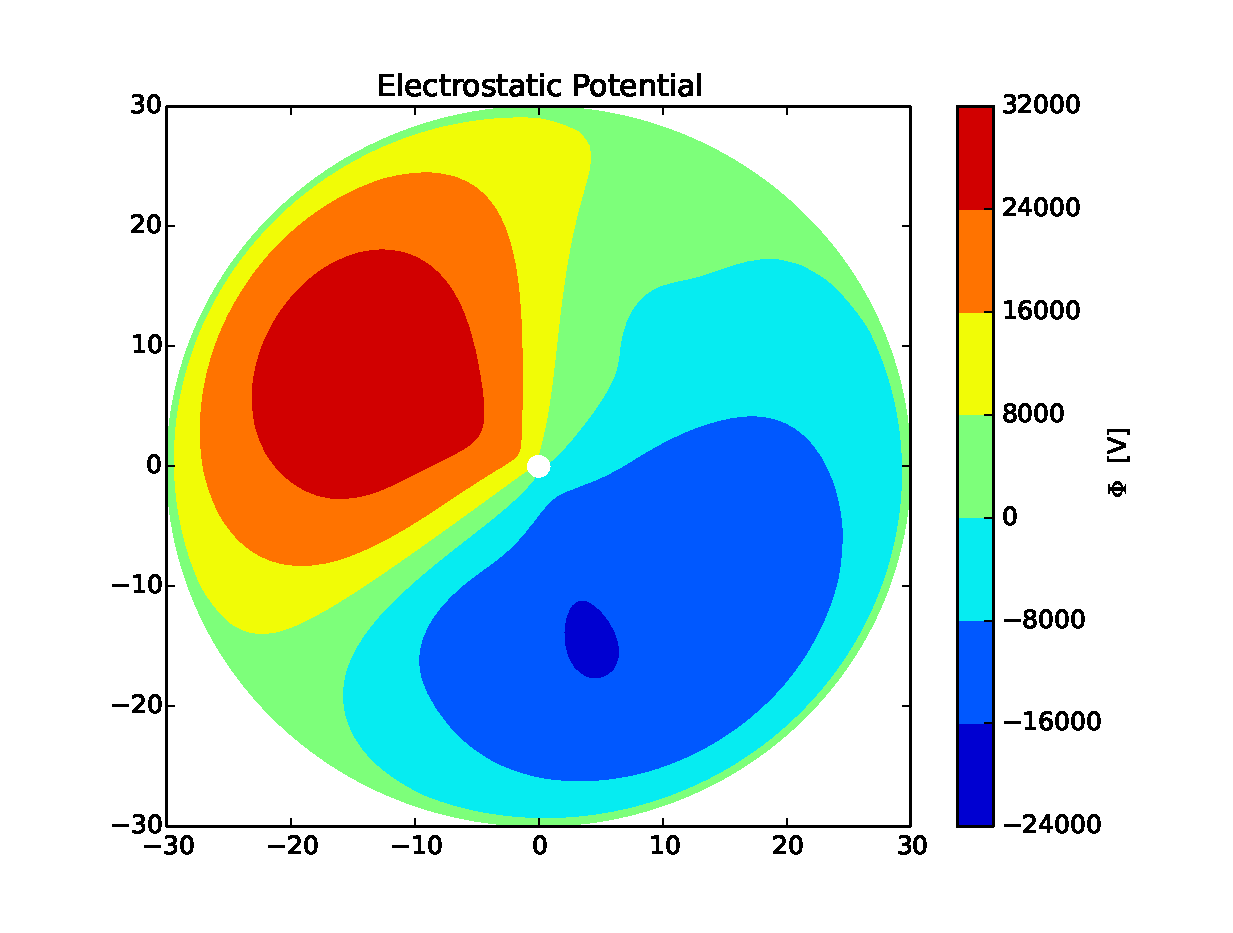
\includegraphics[scale = 0.5]{../source/other_proj}   
    \caption{The electrostatic potential in the higher latitudes.}
    \label{fig:potential}   
  \end{figure}


\appendix
\section{Comments regarding the exercise}
  \begin{itemize}
    \item Is there no scaling factor on the potential? Does the spherical harmonics coefficients have them baked in?
    \item Some efficiency could be obtained by keeping in mind that \(m<\ell\)
    \item I didn't really find any good documentation on the associated legendre function, the official scipy documentation was sparse and wrote the input as lpmv( m (order) , v (degree), x (argument)  ).
          On the other hand I went to the source code and as far as I could read, (don't know fortran), it the input should be lpmv( v, m, x ). \href{https://github.com/scipy/scipy/blob/master/scipy/special/specfun/specfun.f#L7965}{source}, \href{http://docs.scipy.org/doc/scipy/reference/generated/scipy.special.lpmv.html#scipy.special.lpmv} {documentation}.
          \begin{lstlisting}
                    SUBROUTINE LPMV0(V,M,X,PMV)
          C
          C       =======================================================
          C       Purpose: Compute the associated Legendre function
          C                Pmv(x) with an integer order and an arbitrary
          C                nonnegative degree v
          C       Input :  x   --- Argument of Pm(x)  ( -1 <= x <= 1 )
          C                m   --- Order of Pmv(x)
          C                v   --- Degree of Pmv(x)
          C       Output:  PMV --- Pmv(x)
          C       Routine called:  PSI_SPEC for computing Psi function
          C       =======================================================
          \end{lstlisting}
          Not that any changes in the final potential was visible (due to some error or symmetry I would guess), see \cref{fig:potential_wrong}.
      \item I hope that the potential looks ok, I don't really know how it is supposed to look. Quickly checked a \href{https://engineering.dartmouth.edu/~d76205x/research/papers/global/node5.html}{resource} and the order of magnitude and the two poles seems to be correct.
      \item 
  \end{itemize}

  \begin{figure}
    \centering
    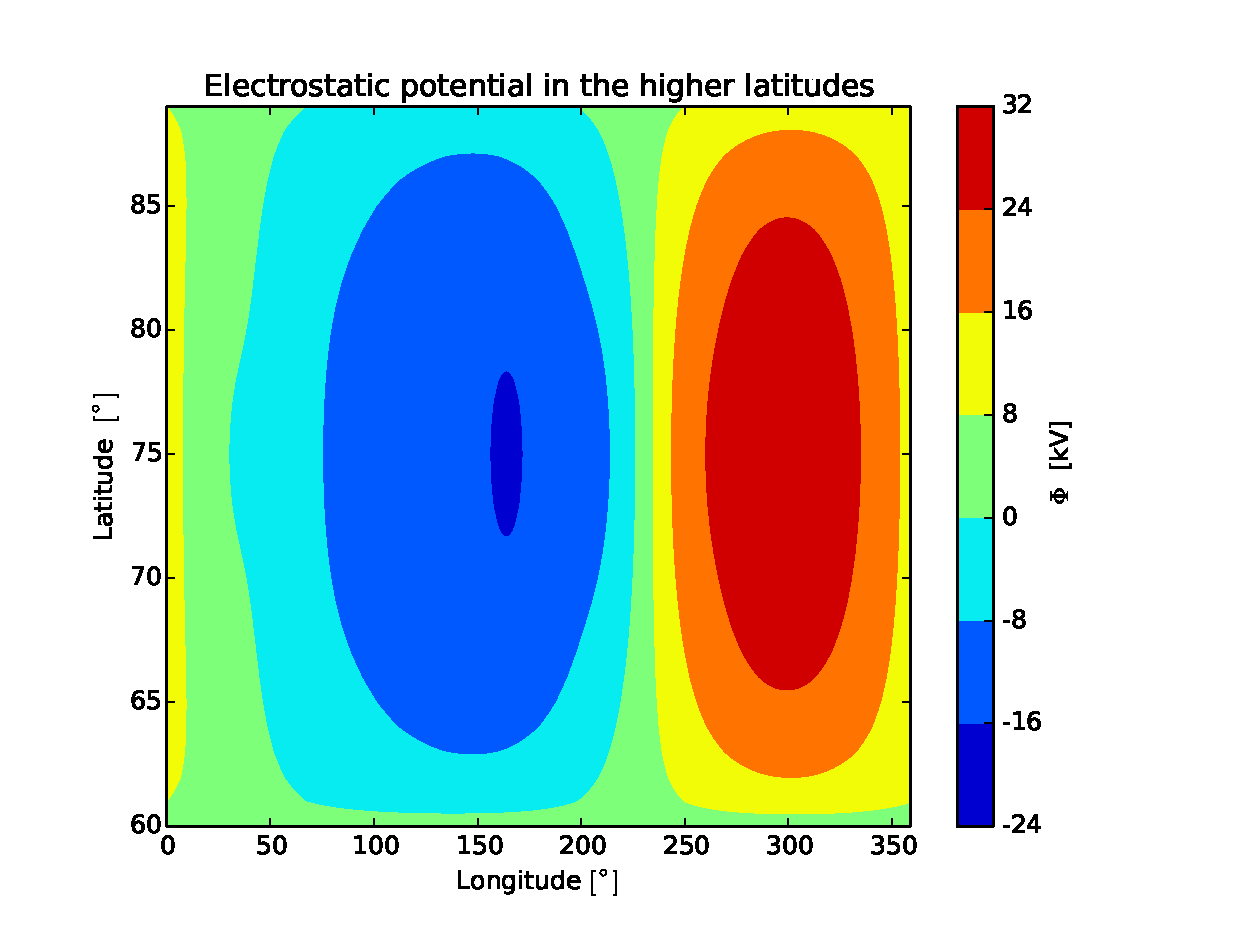
\includegraphics[scale = 0.5]{../source/potential_wrong}
    \caption{Potential with the alternative input to the Legendre function, lpmv( m,l,argument ).}
    \label{fig:potential_wrong}
  \end{figure}

\section{Code}
  \label{sec:code}
  \lstinputlisting{../source/potential_grid.py}

      

\end{document}